\section{Workshop Structure and Methods}
\label{sec:design}

This section describes guidelines for the methods used in the three phases of the \workshop structure (described in Sec.~\ref{sec:process-and-structure}) --- the opening, core, and closing. It concludes with a summary of an example workshop and resources for additional workshop methods.

\subsection{Workshop Opening}

The workshop opening communicates the goals and guidelines for participants, but it can be more than that. It can foster \agency by encouraging self-expression and idea generation. It can encourage \collegiality and \trust by promoting open communication, acknowledging expertise, and establishing a safe co-owned environment. It can also garner \interest by showing that the workshop will be useful and enjoyable. Two guidelines contribute to an effective opening.

\paragraph{Set the stage --- engage.} \workshops typically open with a short introduction that reiterates the theme and establishes shared context for participants and facilitators. We have introduced workshops as \emph{``guided activities that are meant to help us understand: what would you like to do with visualization?''}~[\ref{pro:graffinity}]. We have also used graphics that summarize the goals of our project, potentially priming participants to engage with the \topic of visualization [\ref{pro:htva}].

The opening can establish principles for creativity~\cite{CreativeEducationFoundation2015,Osborn1953}, potentially fostering \trust and \collegiality. We used the following principles in one of our workshops [\ref{pro:eon}]: 1) all ideas are valid, express and record them; 2) let everyone have their say; 3) be supportive of others; 4) instead of criticizing, create additional ideas; 5) think `possibility' -- not implementation; 6) speak in headlines and follow with detail; and 7) switch off all electronic devices.

Introduction presentations should be kept short to maintain \interest. Passive methods, such as lectures and presentations, can discourage participation at the outset. For example, we started one workshop [\ref{pro:arbor}] with a presentation on the current state of analysis tools. This presentation encouraged participants to passively listen rather than actively explore, establishing a passive mindset that we had to overcome in subsequent methods. An effective opening engages participants.

\paragraph{Encourage self-expression.} We use methods that encourage self-expression to support interpersonal leveling and to act on the creativity principles --- {\it all ideas are valid} and {\it be supportive of others}. Such interpersonal methods help to establish an atmosphere of \trust and \collegiality among participants and facilitators. They can also provide participants with a sense of \agency~\cite{Brooks-Harris1999}.

We have used interpersonal methods that ask participants to sketch ideas while suspending judgment~\cite{Rogers2017} or to introduce themselves through analogies as a potential primer for creativity (see analogy introduction in Sec.~\ref{sec:workshop-methods}). Overall, we use interpersonal methods in the opening to engage participants and facilitators, preparing them for the workshop core.

\subsection{Workshop Core}

In the workshop core, we harness the active and engaged mindset of participants by encouraging them to explore a wide ideaspace before selecting the more promising ideas. The methods in the core potentially generate hundreds of sticky notes, sketches, and other artifacts. Analysis of our experience and relevant literature leads us to suggest five guidelines for an effective core.

\paragraph{Elicit visualization opportunities.} We select workshop methods relevant to the \topic, asking participants about their current analysis challenges, limitations of existing tools, characteristics of their data, or the ways in which they would like to use visualization. This can be achieved by adding a visualization twist to existing design and workshop methods. 

In one workshop [\ref{pro:htva}], for example, we used a method that {\it ``developed user stories, considered relevant datasets, discussed alternative scenarios and sketched solutions"} with our domain collaborators. In retrospect, this method connected the \topic into a more general workshop method, user stories~\cite{Kumar2012}.

% More formally, we refer to the set of all ideas being considered in the workshop as the ideaspace~\cite{Biskjaer2017}, and we select or tailor methods that focus on the ideaspace on the \topic --- exploring possibilities for visualization in a domain.

% \paragraph{Elicit relevant ideas.} We refer to the set of all ideas being considered in the workshop as the ideaspace~\cite{Biskjaer2017}. We select methods that focus the ideaspace on the \topic --- exploring the possibilities for visualization in a specific domain.

% In line with existing visualization practices~\cite{Sedlmair2012}, we use methods that ask participants about their problems, not their envisioned solutions. Example prompts of effective methods include {\it ``What would you like to see in your data?''}~[\ref{pro:eon}], and {\it ``What do you want to do with visualization software?''}~[\ref{pro:cp}]. Responses to these prompts help us discover interesting visualization opportunities.

%This requires judgment to balance focus with flexibility. Allowing for freewheeling discussion and ideation can waste time ~\cite{Chamorro-Premuzic2015}, distract from the \topic, and potentially limit \interest. We have seen this in workshops where participants reported that unconstrained discussions were less effective because they allowed for distractions [\ref{pro:arbor}]. Accordingly, we use methods that have been tailored with domain-specific prompts to produce relevant output. As facilitators, this can feel paradoxical. On the one hand, we use workshops to consider a wide range of possibilities and promote serendipitous discovery. But, exploring a wide range of ideas is made possible through methods remain narrowly focused on the \topic. 

%\paragraph{Look for opportunities.} Remember: we use workshops to discover opportunities for visualization research. To this end, we select methods that focus participant energy on communicating their domain challenges, instead of trying to create visualization solutions. We seldom task workshop participants with designing visualizations. We also balance the use of methods that ask directly about visualizations with more open ended questions. For example, we may select methods that ask, {\it ``What would you like to see in your data?''} or {\it ``What are the exceptional characteristics associated with an excellent visualization solution?''} instead of {\it ``What do you want to do with visualization software?''} The differences are subtle, but, in our experience, the former questions elicit what participants need --- the true opportunities for visualization --- instead of what they want.

\paragraph{Explore, then focus.} We organize the core to first generate ideas using divergent methods that expand the ideaspace. Then, we evaluate ideas using convergent methods that winnow the ideaspace~\cite{Osborn1953}. Using divergent methods early in the core allows us to consider many possibilities while also promoting \agency and maintaining \interest. Then, convergent methods can narrow the ideaspace to the more promising ideas. 

Classifying methods as either divergent or convergent risks oversimplification as individual methods often include both divergent and convergent aspects. Consider our use of brainstorming~\cite{Osborn1953} during one workshop~[\ref{pro:edina}]: we asked participants to record \emph{``problems and successes associated with the current clients on \stickyNotes''} (divergent) and then to share the more interesting ideas (convergent). We classify this method as divergent because it creates ideas, despite the convergent discussion. In contrast, a convergent method may only involve grouping \stickyNotes from previous methods. Overall, in line with existing workshop guidance~\cite{CreativeEducationFoundation2015,DeBono1983,Hamilton2016,Osborn1953}, we judge methods by their intended impact on the ideaspace and organize the core with phases of divergent and convergent methods.

\paragraph{Create physical and visual artifacts.} We select methods by how they encourage participants to write, draw, or otherwise externalize their ideas. Externalizing ideas creates artifacts for us to analyze after the workshop. It aids creative thinking because expressing an idea forces the creator to elaborate it~\cite{Sawyer2006}, and promotes idea sharing that encourages \collegiality.

We consider the artifact materials to be important. Sticky notes are particularly useful because they enable participants to group or rank ideas and potentially to discover emergent concepts in the ideaspace~\cite{Dove2016}. We have used \stickyNotes in almost all of our workshops, often using their color to encode information about which method generated an idea, and their positions to relate, differentiate, or rank ideas. This can help establish consensus. It can also aid post-workshop analysis by recording how ideas evolved and were valued throughout the workshop. Additional materials effective for externalizing ideas include handouts with structured prompts, butcher paper, and poster boards. Using whiteboards is tempting, but ideas are easily lost if the boards are erased.

%It also emphasizes the visualization \mindset by using visual \methods.
We also consider the form of ideas to be important. Effective methods create artifacts relevant to the theme and \topic of visualization. This can be achieved through the use of visual language (see wishful thinking in Sec.~\ref{sec:workshop-methods}) and by encouraging participants to sketch or draw, such as in storyboarding [\ref{pro:eon},~\ref{pro:graffinity},~\ref{pro:cp}]. We see many opportunities to create visual artifacts using existing methods, such as sketching with data~\cite{Walny2015}, constructive visualizations~\cite{Huron2014}, or parallel prototyping~\cite{Roberts2016} approaches.

\paragraph{Balance activity with rest.} Because continuously generating or discussing ideas can be tiring for participants, we structure workshop methods to provide a balance between activity and rest. Specifically, we incorporate passive methods that provide time for incubation, the conscious and unconscious combination of ideas~\cite{Sawyer2006}. 

Passive methods can include short breaks with food and coffee, informal discussions over meals, or methods where participants listen to presentations. When using methods that present ideas, asking participants to record their thoughts and reactions can promote \interest and maintain a feeling of \agency. We have typically used passive methods in full-day workshops [\ref{pro:eon},~\ref{pro:graffinity},~\ref{pro:cp},~\ref{pro:arbor}], but we rely on breaks between methods for shorter workshops [\ref{pro:lineage}].

\paragraph{Mix it up.} We consider the relationships among methods to be important as we strive to balance exploration with focus and activity with rest, while also using many materials for externalizing ideas. Considering methods that vary these factors can provide different levels of \challenge because, for example, methods that require drawing ideas may be more difficult than discussing ideas. Using a variety of methods may also maintain \interest because participants may become bored if too much time is spent on a specific idea.

\paragraph{Transition smoothly.} We avoid potentially jarring transitions between methods to preserve participant \interest. Convergent discussions can be used to conclude individual methods by highlighting the interesting, exciting, or influential ideas. These discussions can promote \collegiality by encouraging communication of ideas, \agency by validating participants' contributions, and \interest in the ideas generated. Convergent discussions also highlight potentially important ideas for researchers to focus on after the workshop.

Convergent methods can also conclude the workshop core by grouping or ranking key ideas. We have used storyboarding to encourage the synthesis of ideas into a single narrative [\ref{pro:eon},~\ref{pro:graffinity},~\ref{pro:cp}]. We have also asked participants to rank ideas, providing cues for analyzing the workshop results [\ref{pro:htva}]. Convergent methods provide a sense of validation, potentially helping to build \trust among researchers and collaborators as we transition to the closing. %In our two-day workshop [\ref{pro:arbor}], we concluded the first day by clustering ideas to identify springboards~\cite{Gordon1961} that we explored in the second day. 

\subsection{Workshop Closing}

The workshop closing sets the tone for continued collaboration. It is an opportunity to promote \collegiality by reflecting on the shared creative experience. It allows for analysis that can potentially identify the more interesting visualization opportunities. The following two guidelines apply to effective closings. % by validating the time and energy that participants have contributed, and by identifying the next steps of action.

\paragraph{Encourage reflection for validation.} We use discussions at the end of workshops to encourage reflection, potentially providing validation to participants and generating information valuable for workshop analysis. We encourage participants to reflect on how their ideas have evolved by asking, \emph{``What do you know now that you did not know this morning?''} [\ref{pro:cp}] or \emph{``What will you do differently tomorrow, given what you have learned today?''} [\ref{pro:eon}]. Responses to these questions can provide validation for the time committed to the workshop. One participant, for example, reported, \emph{``I was surprised by how much overlap there was with the challenges I face in my own work and those faced by others''} [\ref{pro:cp}]. 

%Also, because reflective questions are used to start a discussion, they require participants to rank their thoughts and to talk about the more interesting ones. Recording these ideas can provide important clues for the analysis of workshop artifacts, such as in our neuroscience workshop's closing where discussions about \emph{``multi-hop path queries''} resulted in focusing on connectivity analysis [\ref{pro:graffinity}].

\paragraph{Promote continued collaboration.} We conclude the workshop by identifying the next steps of action --- continuing the \methodology of the collaboration. We can explain how the ideas will be used to move the collaboration forward, often with design methods as we describe in Sec.~\ref{sec:after}. 

We can also ask participants for feedback about the workshop to learn more about their perceptions of visualization and to evaluate the effectiveness of workshop methods --- encouraging the visualization mindset. E-mailing online surveys immediately after a workshop is effective for gathering feedback [\ref{pro:graffinity},~\ref{pro:arbor}].

\begin{figure}
    \centering
    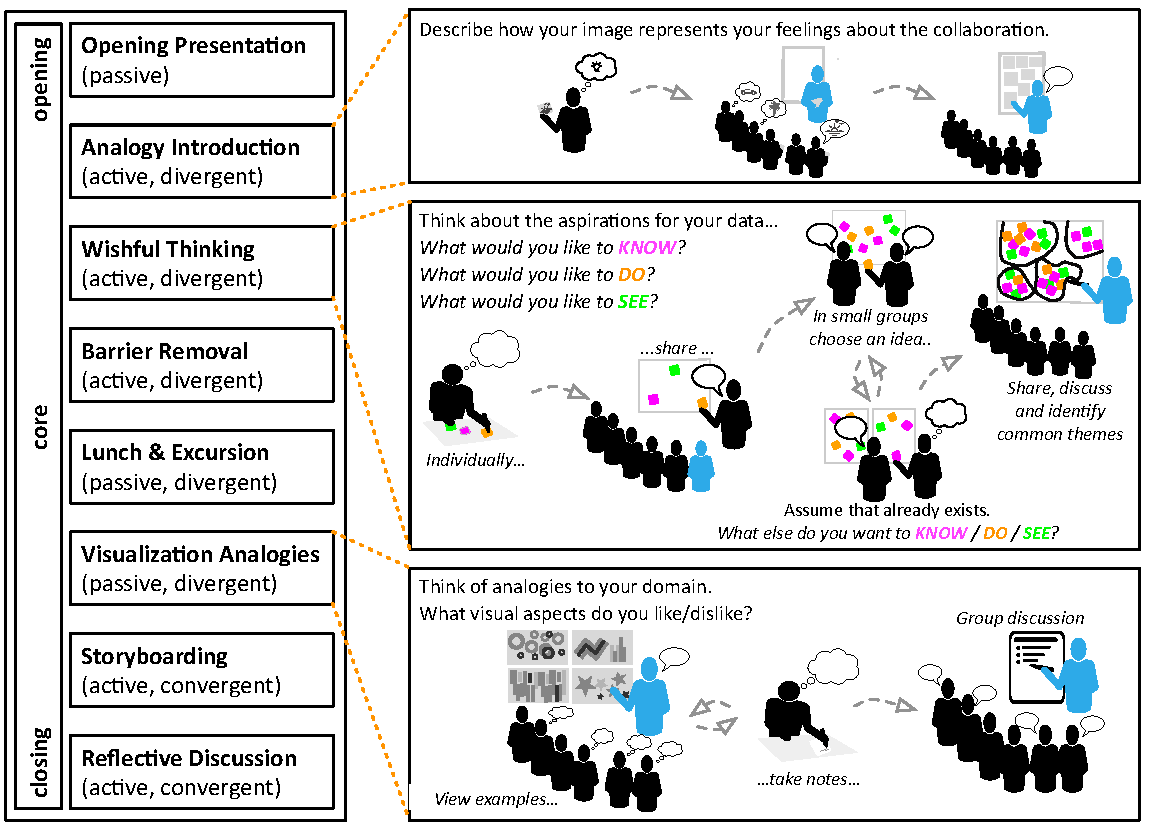
\includegraphics[width=\columnwidth]{figures/workshop.pdf}
    \caption{The eight methods of the full-day, example \workshop (left) with the process of three methods summarized graphically (right). The workshop methods diverge to explore a broad ideaspace before they converge to the more promising ideas. Three of the methods are described in the text and the remainder are explained in the Supplemental Material. The methods can be summarized as: 1) the opening presentation establishes creativity principles; 2) an analogy introduction promotes interpersonal leveling; 3) wishful thinking elicits opportunities for visualization; 4) barrier removal explores those opportunities further; 5) lunch \& excursion provides time for rest and incubation; 6) visualization analogies allows specification of requirements by example; 7) storyboarding summarizes key ideas in a graphic form; and 8) the reflective discussion highlights potentially interesting ideas for workshop analysis. This workshop plan is a starting point for future workshops.}
    \label{fig:example-workshop}
\end{figure}

\subsection{Example Workshop \& Methods}
\label{sec:workshop-methods}
To illustrate the workshop structure, we include an example workshop, shown in Fig.~\ref{fig:example-workshop}. We selected this example because it has proven effective in three of our projects [\ref{pro:eon},~\ref{pro:graffinity},~\ref{pro:cp}]. Here, we describe three methods of this workshop that we have also used successfully in additional workshops [\ref{pro:lineage},~\ref{pro:arbor}], and we refer to the Supplemental Material for descriptions of the remaining five methods. We emphasize that this is a starting place for thinking about workshops, and encourage that methods be adopted and adapted for local context.

To explain the workshop methods, we refer to their process --- the steps of execution~\cite{Biskjaer2017}. This process description abstracts and simplifies the methods because during their execution we adapt the process based on participant reactions and our own judgment of the \tactics. 

\subsubsection*{Analogy Introduction} 

We have used this active, interpersonal, and potentially divergent method in the workshop opening. A process of this method, shown in Fig.~\ref{fig:example-workshop} (right, top), starts with a facilitator posing the analogy introduction prompt, e.g., \emph{``If you were to describe yourself as an animal, what would you be and why?''} [\ref{pro:eon}]. The facilitators and participants then respond to the prompt in turn --- expressing themselves creatively. 

Because everyone responds to the eccentric prompt, this method supports interpersonal leveling that helps to develop \trust and \collegiality among stakeholders. Using analogy can prime participants to think creatively~\cite{Gordon1961}.

This method is simple to execute, and participants report that it has a profound impact on the workshop because of the leveling that occurs. The method helps to establish \trust and that all ideas should be accepted and explored [\ref{pro:graffinity}].

A more topical alternative requires more preparation. We have asked participants to come to the workshop with an image that represents their feelings about the project. Participants have created realistic images, clip-art, and sketches to present and discuss [\ref{pro:htva}]. A visual analogy introduction can help establish the \topic of visualization early in the workshop.

\subsubsection*{Wishful Thinking} 

We have used this divergent, active method early in the workshop core. It is based on creativity methods to generate aspirations~\cite{Hicks2004}. We tailored these methods to visualization by prompting participants with a domain scenario and asking questions: {\it ``What would you like to know? What would you like to do? What would you like to see?''}

One process of this method is shown in Fig.~\ref{fig:example-workshop} (right, middle). First, we introduce the prompt and participants answer the know/do/see questions individually on \stickyNotes. Next, participants share ideas in a large group to encourage \collegiality and cross-pollination of ideas. Then, participants form small groups and try to build on their responses by selecting interesting ideas, assuming that they have been completed, and responding to the know/do/see questions again --- increasing the \challenge. Finally, we lead a convergent discussion to highlight interesting ideas and to transition to the next method.

We encourage participants to record answers to the know/do/see questions on different color \stickyNotes because each prompt provides information that is useful at different points in the design process. Participants describe envisaged insights they would like \emph{to know} and analysis tasks that they would like \emph{to do}. Asking what participants would like {\it to see} is often more of a \challenge, but ensures that a \topic of visualization is established early.

We tailor the prompt to the workshop theme and project goals. For example, we asked energy analysts about long term goals for their project --- \emph{``aspirations for the Smart Home programme\ldots''} They generated forward-thinking ideas, e.g., to better understand the value of the data [\ref{pro:eon}]. In contrast, we asked neuroscientists about their current analysis needs --- \emph{``suppose you are analyzing a connectome\ldots''} They created shorter term ideas, e.g., to see neuron connectivity [\ref{pro:graffinity}].

%The ideas generated in this method can cascade through the workshop. They can be ranked by importance or grouped to find emergent themes. They can also be elaborated in subsequent methods, such as Barrier Removal in the example workshop.

\subsubsection*{Visualization Analogies} 

We have used this divergent, initially passive method later in the workshop core because it promotes incubation while allowing participants to specify visualization requirements by example.  Similar to analogy-based creativity methods~\cite{Gordon1961} and the visualization awareness method~\cite{Koh2011}, we present a curated collection of visualizations and ask participants to individually record analogies to their domain and to specify aspects of the visualizations that they like or dislike. We have used this method repeatedly, iteratively improving its process by reflecting on what worked in a number of our workshops [\ref{pro:edina}~--~\ref{pro:cp},~\ref{pro:arbor}]. 

%  %This activity is low on \collegiality and \challenge but is intended to have positive effects on \trust and \interest.

One process of this method is shown in Fig.~\ref{fig:example-workshop} (right, bottom). First, we provide participants with paper handouts that contain a representative image of each visualization --- we have encouraged participants to annotate the handouts, externalizing their ideas [\ref{pro:graffinity},~\ref{pro:cp},~\ref{pro:arbor}]. Next, we present the curated visualizations on a projector and ask participants to think independently about how each visualization could apply to their domain and record their ideas. Then, we discuss these visualizations and analogies in a large group.

We curate the example visualizations to increase \interest and establish participants' \trust in our visualization expertise. We have used visualizations that we created (to show authority and credibility); those that we did not create (for diversity and to show knowledge of the field); older examples (to show depth of knowledge); challenging examples (to stretch thinking); playful examples (to support engagement and creativity); closely related examples (to make analogies less of a \challenge); and unrelated examples (to promote more challenging divergent thinking).

The discussions during this method have expanded the workshop ideaspace in surprising ways, including \emph{``What does it mean for legends to move?''} [\ref{pro:edina}], \emph{``What does it mean for energy to flow?''} [\ref{pro:eon}], and \emph{``What does it mean for neurons to rhyme?''}~[\ref{pro:graffinity}]. Although this method is primarily passive, participants report that it is engaging and inspiring to see the possibilities of visualization and think about how such visualizations apply to their domain.

% Because this method is initially passive, it gives participants room to think individually. They reported that it is engaging and inspiring to see the broad possibilities of visualization and discuss how such visualizations apply to their domain.

\subsubsection*{Additional Methods \& Resources} 

We introduce the example workshop and methods as starting points for future workshops. Yet, the workshop design space is practically infinite and design should be approached with creativity in mind.

To help researchers navigate the design space, our Supplemental Material contains a list of \numberOfExampleMethods example methods that we have used or would consider using in future workshops. For these methods, we describe their process, their influence on the workshop ideaspace, their level of activity, and their potential impact on the \tactics for effective workshops.

We have also found other resources particularly useful while designing workshops. These include books~\cite{CreativeEducationFoundation2015,Gray2010,Hamilton2016,Hohmann2007,Kumar2012,Michalko2006} and research papers~\cite{McFadzean1998,McKenna2014,Sanders2005}. Although these resources target a range of domains outside of visualization, we tailor the workshop methods such that they encourage a visualization mindset and focus on the \topic of visualization opportunities.